\chapter{Sentinel KMS: Design and Development}\label{ch:system}

\section{Design purpose and use cases}

We developed Sentinel as a knowledge-management system that uses machine learning to support incident analysis and response. It brings together a document library, source ingestion, and a conversational assistant. The purpose is to make applicable knowledge easier to locate, interpret, and reuse when an analyst must decide what to investigate or do next. Embedding models help retrieve relevant passages; a language model uses those passages to explain response options. Publication controls and inspectable evidence connect this assistance to maintained organisational knowledge.

Consider an analyst receiving the report, ``I entered my password after following a suspicious message.'' The useful knowledge may be distributed across a phishing playbook, account-recovery guidance, and a local procedure assigning responsibility for identity administration. Sentinel provides two entry points: the analyst can browse the library directly or describe the situation to the assistant. The assistant receives the observations, retrieves accessible material, and is instructed to distinguish reported facts from possible explanations. The analyst can then open the supporting passages before deciding whether the advice fits the affected service and their authority to act.

This example defines the system's advisory scope. Sentinel supports the interpretation of incident information and the preparation of a response; the responder remains responsible for decisions and changes to operational systems. Knowledge custodians maintain the material on which that assistance depends. Editors propose revisions, administrators control publication, and operators monitor ingestion and service availability. Together, these roles connect knowledge capture and maintenance in RQ1 to contextual, traceable guidance in RQ2. RQ3 concerns how well that design supports retrieval, response quality, task efficiency, and usability.

\section{Requirements and design priorities}

The initial requirements work combined a literature review with semi-structured interviews with a research specialist to identify use cases and user roles. We develop that starting point into four functional requirements and three non-functional requirements in Table~\ref{tab:system-requirements}. The functional requirements follow the movement of knowledge from maintained content to incident guidance. The non-functional requirements apply throughout that movement: access restrictions must survive processing, consequential operations must remain reviewable, and deployment choices must accommodate different hosting constraints.

\begin{table}[htbp]
\centering\small
\caption{Requirements guiding the design of Sentinel.}
\label{tab:system-requirements}
\begin{tabularx}{\textwidth}{@{}>{\raggedright\arraybackslash}p{0.25\textwidth}XX@{}}
\toprule
\rowcolor{TableNavy}
\color{white}\bfseries Requirement & \color{white}\bfseries Intended capability & \color{white}\bfseries Design response \\
\midrule
\rowcolor{TableStripe}
F1 Governed knowledge & Capture, organise, and maintain material suitable for reuse. & Classified articles, immutable revisions, review, publication, and expiry. \\
F2 Recoverable ingestion & Preserve submitted sources and resume interrupted processing. & Retained content, durable jobs, retry, and protected index replacement. \\
\rowcolor{TableStripe}
F3 Contextual retrieval & Locate accessible knowledge relevant to the incident question. & Embeddings, lexical search, indicator lookup, and rank fusion. \\
F4 Traceable incident guidance & Explain response options with inspectable supporting material. & Source-based prompts, playbook fallback, citations, and passage viewing. \\
\rowcolor{TableStripe}
N1 Access and disclosure safety & Respect knowledge restrictions throughout assistance. & Membership and lifecycle checks before retrieval, disclosure, and evidence viewing. \\
N2 Reviewable operations & Retain information needed to investigate system decisions and failures. & Revision history, job states, source references, and redacted audit events. \\
\rowcolor{TableStripe}
N3 Deployment flexibility & Separate infrastructure and model-hosting choices. & Configurable database, identity, chat, and embedding services. \\
\bottomrule
\end{tabularx}
\end{table}

Requirements specify the capabilities we seek; validation criteria specify how we judge them. For example, F2 calls for recoverable ingestion, while a corresponding criterion asks whether recovery uses the retained source and prevents an obsolete worker from replacing newer content. F3 requires contextual retrieval; its evaluation concerns the relevance of returned passages for defined questions. F4 requires traceability, with separate assessment of citation resolution and whether cited passages support the advice. Chapter~\ref{ch:evaluation} connects these criteria to technical checks and the evaluation of analyst-facing tasks. This distinction keeps design choices separate from observed effectiveness.

\section{Architecture and allocation of responsibilities}

Sentinel uses a React interface, a Spring application, and PostgreSQL with pgvector for vector storage. Figure~\ref{fig:sentinel-architecture} shows how these parts connect. The interface presents knowledge and captures requests. The application coordinates publication, ingestion, retrieval, and generation. PostgreSQL retains the knowledge, access rules, processing state, and evidence references needed by those activities. Identity and model services remain separately configurable dependencies.

We place publication rules and assistant orchestration in the same application so that a retrieved passage follows the same access policy as an article opened in the library. Keeping relational and vector data together also allows retrieval to check publication and membership alongside candidate selection. This choice reduces the number of services needed to coordinate evidence eligibility. Its cost is tighter coupling between search and the knowledge schema: changes to classification or lifecycle rules must be reflected consistently in direct reading and retrieval.

The data model separates representations with different purposes. An article provides the current reading view. A revision preserves a particular content state. An evidence snapshot retains the text against which a citation is resolved. Embeddings are derived search representations and can be regenerated without redefining the underlying knowledge. This separation allows an editor to revise guidance while preserving the identity of material previously used in a conversation. A separate assertion store records evidence-linked entities and relationships; the assistant retrieves passages rather than traversing that store.

Long-running work is handled asynchronously. Admission records a source before an ingestion worker extracts and indexes it. Publication records a reindex request in the same transaction as the knowledge change. The browser can therefore distinguish acceptance from subsequent processing, while a restart can recover outstanding work. We accept a delay between publication and search availability in exchange for keeping model calls outside the publication transaction and protecting the identity of the revision being indexed.

\begin{figure}[htbp]
\centering
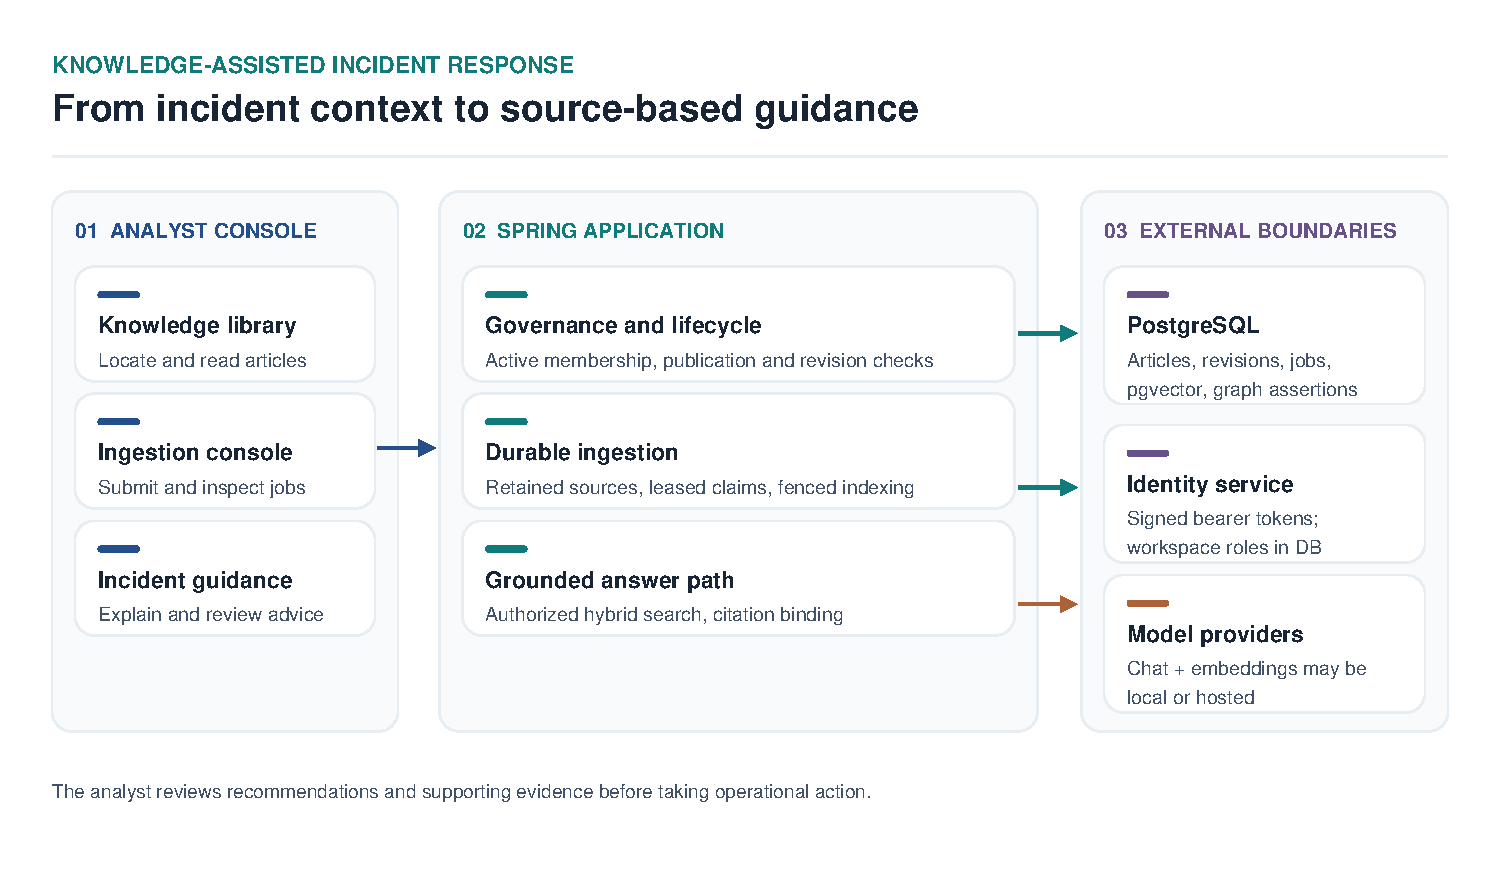
\includegraphics[width=\textwidth]{figures/architecture.pdf}
\caption{Sentinel's knowledge, application, and external-service boundaries.}
\label{fig:sentinel-architecture}
\end{figure}
\FloatBarrier

\section{Knowledge organisation and maintenance}

\subsection{Articles and curated incident playbooks}

The library organises articles by category, severity, tags, source, and update date. Article bodies contain titled sections, with related documents and indicators of compromise where applicable. These fields serve different reading tasks: a category narrows the type of knowledge, a source identifies its origin, and related documents connect an initial observation to further investigation. Severity describes the material's assigned importance; it does not diagnose the incident described by an analyst.

We include a curated collection of response playbooks to give the assistant procedural material alongside advisories and technical descriptions. Its scenarios include phishing, ransomware, account takeover, exposed credentials, application compromise, data exposure, and recovery. Each playbook follows a recognisable structure: applicability, questions to answer, first actions, evidence to preserve, containment and recovery, verification, and escalation. Decision checkpoints explain where context changes the response. For example, the phishing guidance distinguishes receiving a message from entering credentials or executing a downloaded file. We include these distinctions so that retrieved material can address the reported interaction rather than describe the threat only.

The playbooks are source-attributed editorial syntheses, identified as AI-assisted and requiring human review. Their admission checks require attribution, declared categories, consistent identifiers, and the review notice; they also exclude unverified indicators from this general guidance. Installation adds missing articles through the governed publication process and preserves existing content when it differs. A custodian must review such differences rather than lose local adaptations during a refresh. Here, approval permits reference use; operational applicability still depends on review in the receiving organisation.

\subsection{Review, publication, and reuse}

An editor can create a draft revision and submit it for review while the current approved article remains available. Administrative approval rejects self-approval and publishes the accepted revision. Rejection leaves the existing publication intact. State-version checks detect a decision based on an outdated workflow state, which matters when several custodians are maintaining the same procedure. This workflow supports knowledge improvement without making unfinished advice available to the assistant.

Supersession publishes a reviewed successor, whereas administrative rollback creates a new revision from previously published content. Rollback preserves a forward-moving revision history and uses a separate administrative publication route. Expiry removes material from present read eligibility while retaining its history. These operations make maintenance part of knowledge reuse: a response procedure can remain attributable without remaining suitable for current advice.

The publication transaction also records durable reindex work. Replacement is tied to the intended revision and governance state, so a delayed worker cannot publish search material for an obsolete state. During reindexing, an approved revision may temporarily lack searchable embeddings. We favour this gap over allowing superseded guidance to enter a new answer simply because its vectors are still stored.

We keep saved answers separate from published guidance. A conversation can support follow-up work, while knowledge custodians decide which lessons belong in a revised article. This separation prevents a generated response from acquiring publication authority merely because it has been retained. Reuse therefore depends on editorial judgement as well as the ability to search prior knowledge.

\subsection{Maintaining externally supplied knowledge}

Source connectors complement local material with vulnerability and incident information. Refreshes for NVD, CISA KEV, and SANS ISC use persisted work queues, progress records, and source checkpoints. Unchanged records retain their revision; changed source-owned records receive new revisions and evidence. Manual policy or content changes require review instead of being silently overwritten by a feed. Fetching and reindexing remain separate stages, so connector progress and search readiness answer different operational questions.

Trusted producers can publish reference material through an explicit admission route without manual review of each item. This is a decision about which producers the KMS accepts, with the corresponding maintenance responsibility assigned to its operators. Together with the curated collection and editor-managed articles, it gives the library several acquisition routes while retaining a common publication and evidence model.

\section{Recoverable ingestion of local and remote sources}

Incident knowledge also arrives as uploaded documents or material imported from a URL. Sentinel checks uploads for accepted formats and size, assigns source identities, and retains their content before exposing a queued job. URL admission checks the destination; the worker retains the first successful response before extraction. A retry consequently processes the same retained material rather than relying on an open browser session or downloading an unnoticed replacement. Optional owner-scoped request identifiers allow repeated submissions of the same request to recover its existing job.

Processing separates extraction, sanitisation, chunking, embedding, and indexing. For uploaded text, the configured chunker uses character windows of 1200 characters with an overlap of 150. Overlap retains some context across boundaries, while fixed windows keep processing predictable across document formats. The tradeoff is that a window may divide a sentence or procedure. Governed articles instead provide retained evidence passages with explicit identities. Missing source content or empty extraction produces a failed job that can be inspected and, when appropriate, retried.

A worker holds a time-limited claim with a token and processing generation. Progress updates and index replacement must match that live claim. Recovery advances the generation, preventing a delayed worker from overwriting a later retry or restoring deleted material. Repeated embedding calls remain possible when a worker loses its claim after contacting a provider; the protected operation is the replacement of searchable content. This design addresses F2 by preserving continuity of knowledge acquisition through interruptions.

An indexed upload retains its own access scope and processing history. Indexing alone does not turn it into an approved library article. The assistant can use an authorised upload as grounding, but article publication and article-level citations require their corresponding evidence identities. Keeping these routes distinct allows an analyst to consult submitted material without making it organisational guidance by accident.

\section{Machine-learning retrieval and incident guidance}

The assistant follows retrieval-augmented generation (RAG): it retrieves knowledge for the reported situation and supplies that material to a language model. We use machine learning for representation and explanation, while explicit application rules determine which knowledge is eligible and how its use can be inspected.

\subsection{Combining semantic and lexical retrieval}

Machine learning enters retrieval through embeddings: numerical representations of passages and questions produced by an embedding model. Sentinel compares the question representation with stored passage vectors using cosine distance. We use this route to address differences between the language of a report and the terminology of the library. A person may describe encrypted files without naming the relevant response category. Lexical search supplies a complementary route for terms and identifiers that appear explicitly in the question and stored text.

Both searches apply article eligibility and access conditions before limiting their candidate lists. Eligible article passages belong to the current approved, active, unexpired revision and match a retained evidence span. Upload candidates follow their durable-source access rules. Filtering at this point allows accessible material to compete for the available positions instead of first filling them with inaccessible matches. If vector retrieval fails, lexical retrieval still applies the same access conditions.

We combine the two ranked lists using reciprocal-rank fusion~\cite{cormack2009rrf}. For passage $d$, the ordering score is
\begin{equation}
 F(d)=\sum_{\ell\in\{\mathrm{vector},\mathrm{lexical}\}:d\in\ell}
 \frac{1}{60+\operatorname{rank}_{\ell}(d)}.
\end{equation}
The configured fusion constant is 60; ranks begin at one. This choice combines positions rather than treating cosine similarity and lexical relevance as directly comparable quantities. A passage found by both methods accumulates a contribution from each list. The score determines ordering, not the probability that advice is correct. The configured minimum similarity applies to vector candidates, while category and minimum-severity filters use article metadata in both searches.

\subsection{Establishing the context for an answer}

The assistant supplements hybrid retrieval with access-aware indicator lookup. This gives literal technical observations a route to matching knowledge alongside the broader semantic search. Indicator lookup uses the original question and is separate from the hybrid search's category and severity filters. Its evidence span identifies the indicator occurrence; a surrounding summary still needs to be checked against the full article. After combining candidates, the application resolves readable articles and exact evidence references before constructing model context. An optional reranker receives only authorised candidates.

Conversational rewriting can turn a follow-up question into a standalone search question using recent turns. We place this step after literal-question retrieval has established usable evidence. If that initial retrieval is empty, the assistant returns a local message directing the analyst to refine the question or browse playbooks. This conservative ordering avoids a generated answer detached from accessible knowledge, although it can also leave a context-dependent follow-up unanswered. The question may already have reached the embedding provider during retrieval; the gate controls the subsequent rewriting, reranking, and answer-generation stages.

The prompt combines the question, bounded recent conversation, and selected sources. Each article passage carries source information and a server-issued evidence token. The source-context budget limits prompt growth, at the cost of potentially truncating the final passage. We therefore treat retained grounding references as the material selected for context, rather than a record of the model's reasoning. Knowledge remains external to the generation model: revisions can change what is retrieved without retraining it.

\subsection{Turning retrieved knowledge into response guidance}

We shape the generation instructions around the decisions an incident responder faces. For suspected incidents, the model is asked to separate observations from explanations and organise supported advice around immediate actions, investigation and evidence preservation, recovery, and verification. The instructions call for an explanation of each action's purpose, expected result, and responsible actor. They limit clarification to three focused questions and prohibit assumptions about the operating system, affected platform, or responder's administrative access.

The instructions also require the model to explain operational impact before disruptive actions and to preserve evidence before cleanup. Requests for redacted observations replace requests for passwords, secret keys, verification codes, or complete sensitive logs. A conceptual question can receive a short explanation instead of a forced incident checklist. These instructions define the intended assistance; the reviewable sources and subsequent answer assessment remain necessary because a language model can misapply them.

The application supports structured answer blocks and a natural-language conversation route. Both use the same practical guidance and authorised context. The model is instructed to copy evidence tokens supplied by the server. Response processing resolves accepted tokens to retained references and removes unsupported citation tokens. Article citations and exact-passage references are then associated with the assistant message, making the advice available for later inspection.

\subsection{Useful behaviour when generation is unavailable}

A model failure need not remove access to existing guidance. When generation fails or is temporarily blocked, Sentinel first looks for an eligible playbook among the retrieved articles. It independently resolves up to three bounded sections titled \emph{First actions}, \emph{Questions to answer}, and \emph{Evidence to preserve} from that playbook's current approved revision. The section text comes from retained evidence, with a separate access check for each passage, rather than from trusting the retrieval metadata alone.

The fallback quotes these sections and labels them as existing playbook guidance, not a personalised answer. If section expansion cannot be authorised, it provides available retrieved article references for direct reading. It does not combine fragments into a locally invented response plan. This behaviour preserves a useful part of the KMS during a generation outage while making the loss of contextual adaptation visible. The same final authorisation and citation-persistence checks apply to fallback and generated responses.

\subsection{Keeping guidance attached to evidence}

An exact article citation identifies the article, revision identity and number, evidence snapshot, and passage boundaries. Retrieval checks the passage against the retained snapshot. Figure~\ref{fig:evidence-path} follows this relationship through to inspection. An article title alone would be insufficient because the displayed article could change after the answer was produced. Retaining a passage identity makes that change distinguishable from the evidence originally selected.

Before releasing an answer, the application checks that its grounding remains authorised and persists its references. The conversation route buffers generated output before sending its server-sent events, allowing this final disclosure check to occur before text reaches the browser. The tradeoff is a longer wait for the first visible answer rather than immediate provider-token display.

Evidence inspection performs another current-access check. Superseded, expired, revoked, or otherwise unavailable references return an unavailable state, while their identities can remain in the conversation record. We prioritise present disclosure rules over unrestricted replay of previously visible passages. A resolved citation establishes which material can be inspected; deciding whether that material supports the recommendation remains an analyst and evaluation task.

\begin{figure}[htbp]
\centering
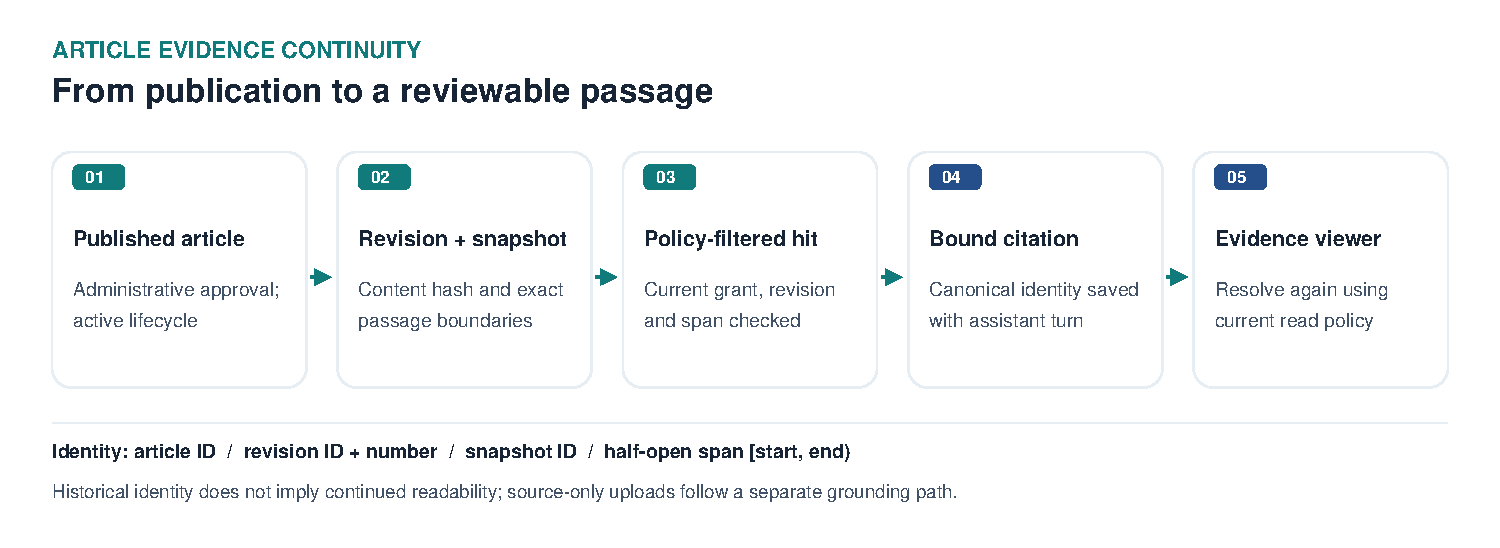
\includegraphics[width=\textwidth]{figures/evidence-path.pdf}
\caption{An editor-managed article's path from publication to access-checked evidence inspection.}
\label{fig:evidence-path}
\end{figure}
\FloatBarrier

\section{Analyst interaction and knowledge reuse}

The interface connects direct reading with conversational assistance. In the knowledge library, topic shortcuts lead to playbooks for recognisable problems such as suspicious messages, encrypted files, compromised accounts, and exposed secrets. Search, category and severity filters, and sorting support more deliberate exploration. An article opens in a reading pane with its sections, source information, and related documents. For playbooks, an action transfers a request to the assistant to help apply the selected guidance, asking about the situation and actions already taken.

The assistant accepts free-text questions and provides an optional response-plan intake. The intake asks what happened, which devices, accounts, or services are affected, and what the reporter has already done. It turns those observations into a structured question requesting priorities, evidence preservation, recovery, verification, and escalation. Unknown fields remain explicitly unknown. This design gives the retrieval and generation stages more context without forcing the reporter to classify the incident before asking for help.

Saved conversations support follow-up and handover; answers can be copied, exported, and rated for usefulness. The response separates article navigation from exact-evidence inspection. Opening a source provides broader reading, whereas the passage action opens the cited revision and span. The dialog checks that the returned identity matches the request and manages keyboard focus while open. This distinction supports both understanding the procedure and checking the specific material associated with an answer.

The ingestion view presents source submission, processing stages, job status, retry controls, and connector refresh. These controls expose the difference between adding material and having it ready for retrieval. Figures~\ref{fig:knowledge-ui}--\ref{fig:evidence-ui} illustrate selected interface states using the actual frontend with deterministic mocked authentication and application responses. Their article text, answers, passages, and counters are demonstration data, not corpus measurements, model results, or observations from an analyst study.

\begin{figure}[htbp]
\centering
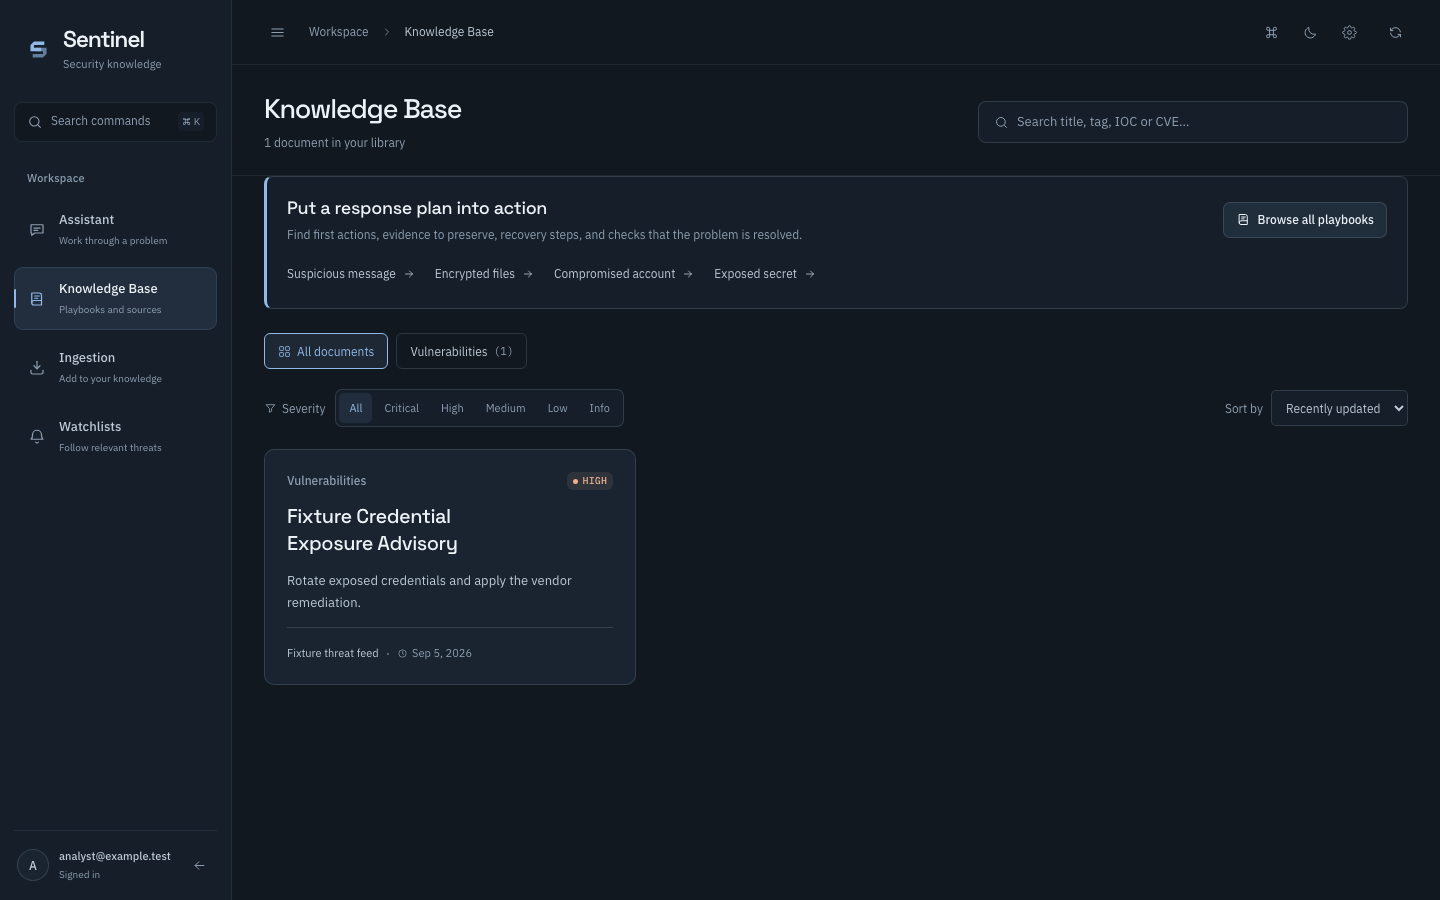
\includegraphics[width=\textwidth,trim=230bp 155bp 15bp 65bp,clip]{figures/main-knowledge-base-mocked.png}
\caption[Knowledge-library filters and playbook browsing (mocked data).]{Knowledge-library filters and problem-oriented playbook browsing (mocked data).}
\label{fig:knowledge-ui}
\end{figure}

\begin{figure}[htbp]
\centering
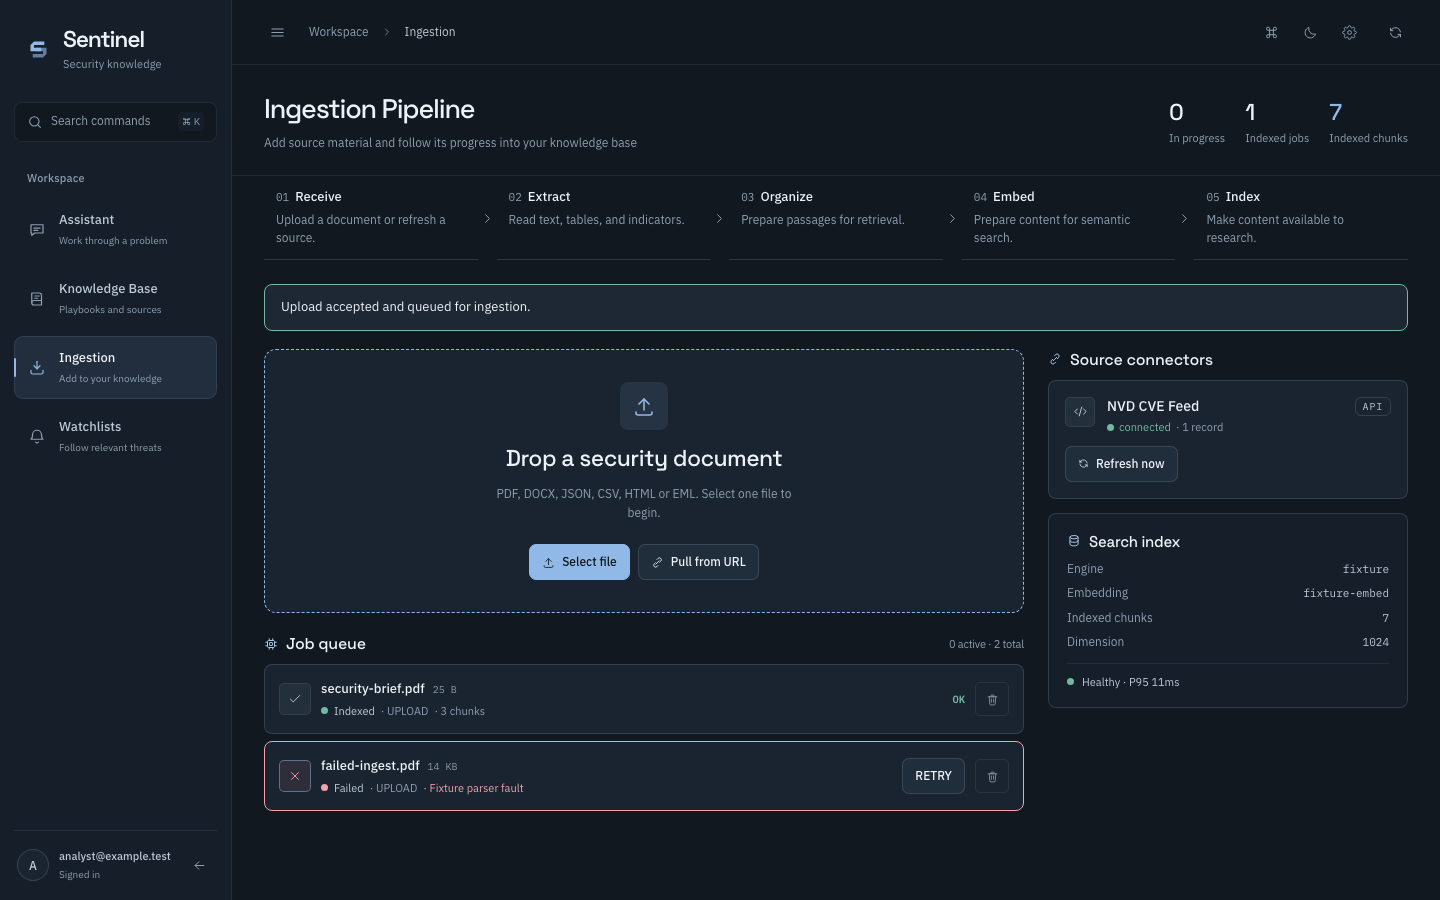
\includegraphics[width=\textwidth,trim=230bp 560bp 15bp 65bp,clip]{figures/main-ingestion-mocked.png}
\caption{Ingestion stages and source-submission acknowledgement (mocked data).}
\label{fig:ingestion-ui}
\end{figure}

\begin{figure}[htbp]
\centering
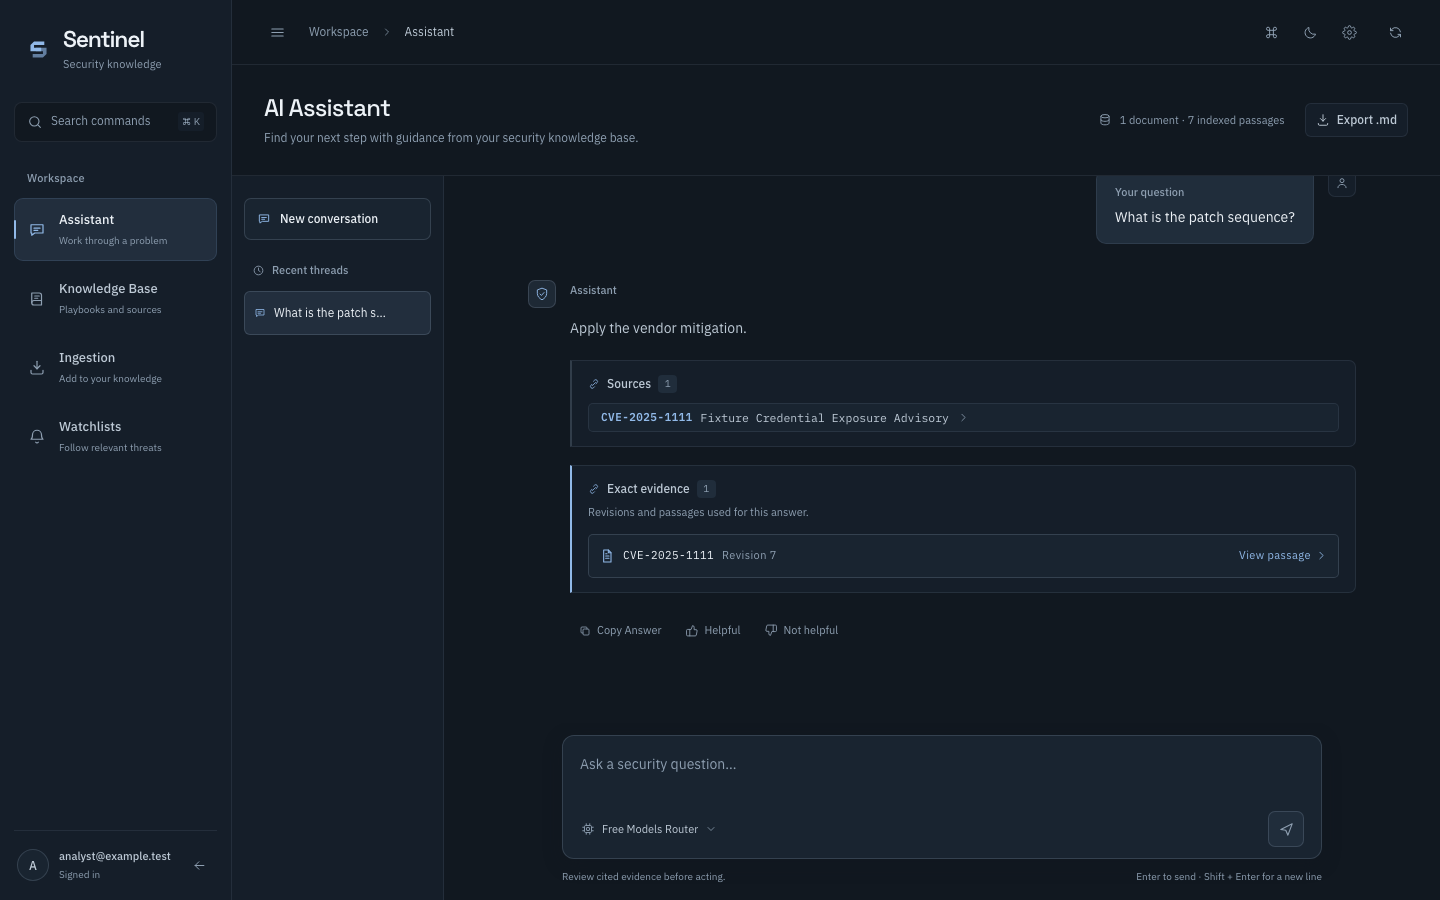
\includegraphics[width=\textwidth,trim=440bp 220bp 60bp 175bp,clip]{figures/main-cited-answer-mocked.png}
\caption{Assistant answer with article and exact-passage actions (mocked data).}
\label{fig:assistant-ui}
\end{figure}

\begin{figure}[htbp]
\centering
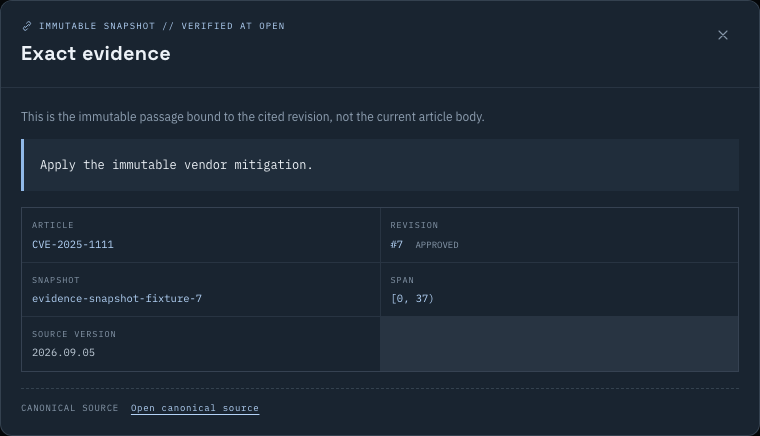
\includegraphics[width=0.85\textwidth]{figures/main-evidence-detail-mocked.png}
\caption{Evidence dialog identifying the cited revision and passage (mocked data).}
\label{fig:evidence-ui}
\end{figure}
\FloatBarrier

\section{Confidentiality and operational choices}

Access policy supports knowledge sharing at different levels. Public articles require authentication; internal material requires workspace membership; confidential and restricted material require editor and administrator authority respectively. Active database memberships determine those roles. Missing or inconsistent governance results in denial. These controls apply to direct reading, retrieval, and evidence disclosure, so a conversational request does not provide an alternative route around the library's restrictions.

Retrieved content is treated as untrusted data. Sanitisation targets recognisable injection patterns before uploaded text is indexed and before source text enters a prompt. The prompt distinguishes source material from instructions. These defences reduce exposure to known patterns but require adversarial evaluation, particularly when unfamiliar documents are admitted. The separation of source permissions from text and metadata remains necessary even when sanitisation leaves a passage apparently harmless.

For N2, revision and workflow histories describe knowledge changes, while job records explain processing progress. Redacted audit events record consequential operations and outcomes. Successful transactional changes produce their success events after the transaction completes. Audit persistence is best-effort: an audit failure is logged without replacing the original operation's result. This favours service continuity but leaves a completeness limitation that operators must consider when investigating an incident involving the KMS itself.

For N3, chat and embedding services can use hosted providers or local models through Ollama. Database and identity hosting are configured separately. Choosing local inference therefore addresses model processing, while the complete disclosure boundary also depends on where knowledge and identity services run. Hosted embedding requests transmit passage or question text; hosted answer requests transmit the question, selected context, and recent conversation. Access eligibility within the KMS and permission to send material to a provider are separate deployment considerations.

The vector store expects 1024-dimensional embeddings. Replacing the embedding model requires reindexing; a different dimensionality also requires a storage change. Reproducibility and confidentiality depend on these deployment choices, not only on the chat model.

\section{Chapter synthesis}

Sentinel connects knowledge acquisition, retrieval and response guidance. Playbooks supply procedures; embeddings and lexical search locate passages; generation relates them to the incident. Direct reading and fallback preserve access when generation fails. Chapter~\ref{ch:evaluation} examines this design against its requirements, distinguishing technical operation from the quality and usefulness of the assistance.
